%==============================常用宏包、环境==============================%
\documentclass[landscape,twocolumn,a4paper]{article}
\usepackage{xeCJK} % For Chinese characters
\usepackage{amsmath, amsthm}
\usepackage{listings,xcolor}
\usepackage{geometry} % 设置页边距
\usepackage{fontspec}
\usepackage{graphicx}
\usepackage{fancyhdr} % 自定义页眉页脚
\usepackage{makecell}
\usepackage[breaklinks,colorlinks,linkcolor=black,citecolor=black,urlcolor=black]{hyperref}
\setsansfont{Consolas} % 设置英文字体
\setmonofont[Mapping={}]{Consolas} % 英文引号之类的正常显示,相当于设置英文字体
\geometry{left=1cm,right=1cm,top=2cm,bottom=2cm} % 页边距
\setlength{\columnsep}{30pt}
% \setlength\columnseprule{0.4pt} % 分割线

\usepackage{xunicode, xltxtra} 
\setmainfont{Microsoft YaHei} 
\usepackage{setspace}
\usepackage{ctex} 
\usepackage[Glenn]{fncychap}
\usepackage{color}
\usepackage{verbatim}



%==============================常用宏包、环境==============================%
\newfontfamily\monaco{Monaco}
\definecolor{dkgreen}{rgb}{0,0.6,0}
\definecolor{gray}{rgb}{0.5,0.5,0.5}
\definecolor{mauve}{rgb}{0.58,0,0.82}

%==============================页眉、页脚、代码格式设置==============================%
% 页眉、页脚设置
\pagestyle{fancy}
% \lhead{CUMTB}
\lhead{\CJKfamily{hei} Standard Code Library}
\chead{}
% \rhead{Page \thepage}
\rhead{\CJKfamily{hei} 第 \thepage 页}
\lfoot{} 
\cfoot{}
\rfoot{\CJKfamily{hei} 第 \thepage 页}
\renewcommand{\headrulewidth}{0.4pt} 
\renewcommand{\footrulewidth}{0.4pt}

\lstset{
    language    = c++,
    numbers     = left,
    numberstyle = \tiny,
    breaklines  = true,
    captionpos  = b,
    tabsize     = 4,
    frame       = simple,
    columns     = fullflexible,
    commentstyle = \color{gray},
    keywordstyle = \bfseries\monaco,
    basicstyle   = \monaco,
    stringstyle  = \color[RGB]{148,0,209}\ttfamily,
    rulesepcolor = \color{red!20!green!20!blue!20},
    showstringspaces = false,
}
%==============================页眉、页脚、代码格式设置==============================%

%==============================标题和目录==============================%
\title{\CJKfamily{hei} \bfseries Standard Code Library}
\author{Xavier\_Cai}
\renewcommand{\today}{\number\year 年 \number\month 月 \number\day 日}

\begin{document}\small
\begin{titlepage}
\maketitle
\end{titlepage}

\newpage
\pagestyle{empty}
\renewcommand{\contentsname}{目录}
\tableofcontents
\newpage\clearpage
\newpage
\pagestyle{fancy}
\setcounter{page}{1}   %new page

%==============================标题和目录==============================%

\section{数据结构}

\subsection{01字典树}

\subsubsection{路径为点权异或值求最小生成树(CF888G)}
\begin{table}[h]
    \begin{tabular}{ll}
        \hline
        \thead[l]{input} & \thead[l]{output} \\
        \hline
        4  \\ 1 2 3 4 &  8 \\
        \hline       
    \end{tabular}
    \label{bs}
\end{table}
\lstinputlisting{数据结构/01字典树/路径为点权异或值求最小生成树(CF888G).cpp}

\subsubsection{可持久化01字典树}
初始有$n$个数,有$m$个操作:\par
\textbf{1 A x} 添加操作,表示在序列末尾添加一个数 $x$ ,序列的长度 $n+1$\par
\textbf{Q l r x} 询问操作,你需要找到一个位置 $p$ ,满足$l \le p \le r$,使得:$ a[p] \oplus a[p+1] \oplus ... \oplus a[N] \oplus x$最大,输出最大是多少。
\lstinputlisting{数据结构/01字典树/可持久化01字典树.cpp}

\subsection{吉司机线段树}

\subsubsection{区间取$min$+区间查询$O(m \log n)$}
\lstinputlisting{数据结构/JLS树/区间求min区间查询.cpp}

\subsubsection{支持区间加(BZOJ4695 最假女选手)$O(m \log ^{2}n)$}
\lstinputlisting{数据结构/JLS树/区间加.cpp}

\subsubsection{维护区间最值操作与区间历史最值(洛谷 线段树$3$)$O(m \log ^{2}n)$}
给出一个长度为 $n$ 的数列 $A$,同时定义一个辅助数组 $B$,$B$ 开始与 $A$ 完全相同。接下来进行了 $m$ 次操作,操作有五种类型,按以下格式给出:\par
\textbf{1 l r k} 对于所有的 $i\in[l,r]$,将 $A_i$ 加上 $k$($k$ 可以为负数)。\par
\textbf{2 l r v} 对于所有的 $i\in[l,r]$,将 $A_i$ 变成 $\min(A_i,v)$。\par
\textbf{3 l r} 求 $\sum_{i=l}^{r}A_i$。\par
\textbf{4 l r} 对于所有的 $i\in[l,r]$,求 $A_i$ 的最大值。\par
\textbf{5 l r} 对于所有的 $i\in[l,r]$,求 $B_i$ 的最大值。\par
在每一次操作后,我们都进行一次更新,让 $B_i\gets\max(B_i,A_i)$。\par
\lstinputlisting{数据结构/JLS树/区间最值操作与区间历史最值.cpp}

\subsection{二维树状数组}

\subsubsection{单点修改+区间查询}
\lstinputlisting{数据结构/二维树状数组/单点修改+区间查询.cpp}

\subsubsection{区间修改+单点查询}
\lstinputlisting{数据结构/二维树状数组/区间修改+单点查询.cpp}

\subsubsection{区间修改+区间查询}
\lstinputlisting{数据结构/二维树状数组/区间修改+区间查询.cpp}

\subsection{二维线段树}
\lstinputlisting{数据结构/二维线段树/单点修改+区间查询.cpp}

\subsection{左偏树(可并堆)}

\subsubsection{左偏树$O(\log n)$}
\lstinputlisting{数据结构/左偏树/LT.cpp}

\subsubsection{带push\_down操作的左偏树子树节点合并([JLOI2015]城池攻占)}
\lstinputlisting{数据结构/左偏树/带push_down操作的左偏树子树节点合并([JLOI2015]城池攻占).cpp}

\subsection{扫描线}

\subsubsection{矩形并面积}
\lstinputlisting{数据结构/扫描线/矩形并算面积.cpp}

\subsubsection{矩形并周长}
\lstinputlisting{数据结构/扫描线/矩形并周长.cpp}

\subsubsection{矩阵求和最值(POJ-2482)}
不含边框注意!
\begin{table}[h]
    \begin{tabular}{ll}
        \hline
        \thead[l]{input} & \thead[l]{output} \\
        \hline
        2 & \\
        3 5 4 & 5\\
        1 2 3 & \\
        2 3 2 & \\
        6 3 1 & \\
        3 5 4 & 6 \\
        1 2 3 & \\
        2 3 2 & \\
        5 3 1 & \\
        \hline       
    \end{tabular}
    \label{bs}
\end{table}
\lstinputlisting{数据结构/扫描线/矩阵求和最值(POJ-2482).cpp}

\subsubsection{旋转扫描线}
含边框注意!
\begin{figure}[htb]
\center{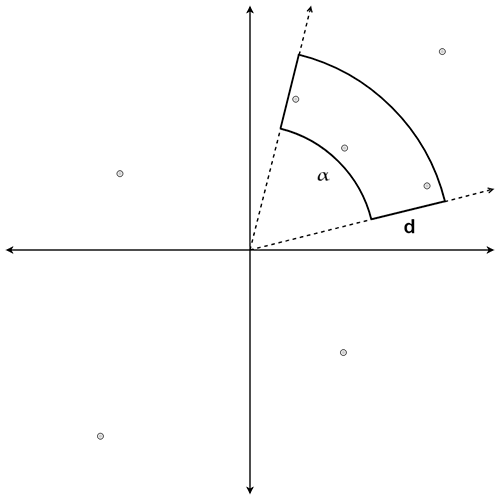
\includegraphics[width=6cm]  {数据结构/扫描线/旋转扫描线pic.jpg}}
\end{figure}
\lstinputlisting{数据结构/扫描线/旋转扫描线.cpp}



\subsection{李超线段树}

\subsubsection{李超上树([SDOI2016]游戏)$O(m \log ^{3}n)$}
有时,$Alice$ 会选择一条从 $s$ 到 $t$ 的路径,在这条路径上的每一个点上都添加一个数字。对于路径上的一个点 $r$,若 $r$ 与 $s$ 的距离是 $dis$,那么 $Alice$ 在点 $r$ 上添加的数字是 $a\times dis + b$。\par
有时,$Bob$ 会选择一条从 $s$ 到 $t$ 的路径。他需要先从这条路径上选择一个点,再从那个点上选择一个数字。\par
$Bob$ 选择的数字越小越好,但大量的数字让 $Bob$ 眼花缭乱。$Bob$ 需要你帮他找出他能够选择的最小的数字。
\lstinputlisting{数据结构/李超线段树/李超上树.cpp}

%================================杂项================================%
\section{杂项}

\subsection{数列归纳}

$f(n) = \frac{(2*n + 1)!}{(n + 1)}$\par
1, 3, 40, 1260, 72576, \par
6652800, 889574400, 163459296000, 39520825344000, 12164510040883200, \par
4644631106519040000, 2154334728240414720000, 1193170003333152768000000, 777776389315596582912000000\par

~\\

$f(n) = \sum_{i=1}^{n} p, p \in prime$\par
转$min_25筛$\par
0, 2, 5, 10, 17, 28, 41, 58, 77, 100, \par
129, 160, 197, 238, 281, 328, 381, 440, 501, 568, \par
639, 712, 791, 874, 963, 1060, 1161, 1264, 1371, 1480, \par
1593, 1720, 1851, 1988, 2127, 2276, 2427, 2584, 2747, 2914, \par
3087, 3266, 3447, 3638, 3831, 4028, 4227, 4438, 4661, 4888\par
\par



\subsection{全1矩阵个数(51nod1291)}
\begin{table}[h]
    \begin{tabular}{ll}
        \hline
        \thead[l]{input} & \thead[l]{output} \\
        \hline
        3 3 & \\
        011 & 6 3 0\\
        110 & 3 1 0\\
        100 & 1 0 0\\
        \hline       
    \end{tabular}
    \label{bs}
\end{table}
\lstinputlisting{杂项/全1矩阵个数(51nod1291).cpp}


%==============================习题整理==============================%
\section{习题整理}

\subsection{可重边集的点能否和当前询问边构成三角形(20牛客2H)(动态点开线段树)}
\begin{table}[h]
    \begin{tabular}{ll}
        \hline
        \thead[l]{input} & \thead[l]{output} \\
        \hline
        8   & \\
        1 1 & \\
        3 1 & No \\
        1 1 & \\
        3 2 & No \\
        3 1 & Yes \\
        1 2 & \\
        2 1 & \\
        3 1 & No \\
        \hline       
    \end{tabular}
    \label{bs}
\end{table}
\lstinputlisting{习题整理/可重边集的点能否和当前询问边构成三角形(20牛客2H)(动态点开线段树).cpp}

\subsection{左偏树离线处理查询成立最多数(HDU5575)}
$0$代表没有水,$1$代表有水\par
\begin{table}[h]
    \begin{tabular}{ll}
        \hline
        \thead[l]{input} & \thead[l]{output} \\
        \hline
        3 4   & 3 \\
        3 4 & \\
        1 3 1 & \\
        2 1 0 & \\
        2 2 0 & \\
        3 3 1 & \\
        \hline       
    \end{tabular}
    \label{bs}
\end{table}
\lstinputlisting{习题整理/左偏树离线处理查询成立最多数(HDU5575).cpp}


\end{document}